\subsection{Tối ưu thông lượng blockchain qua Batch}

\subsubsection{Cơ chế cắt khối của Fabric}

Hyperledger Fabric không đóng khối cho từng giao dịch riêng lẻ mà \textbf{gom nhóm} các giao dịch thành lô tại tầng Orderer. Tham số \pkg{BatchSize} và \pkg{BatchTimeout} trong tệp cấu hình \pkg{configtx.yaml} quyết định khi nào một lô được đóng thành khối:

\begin{figure}[H]
    \centering
    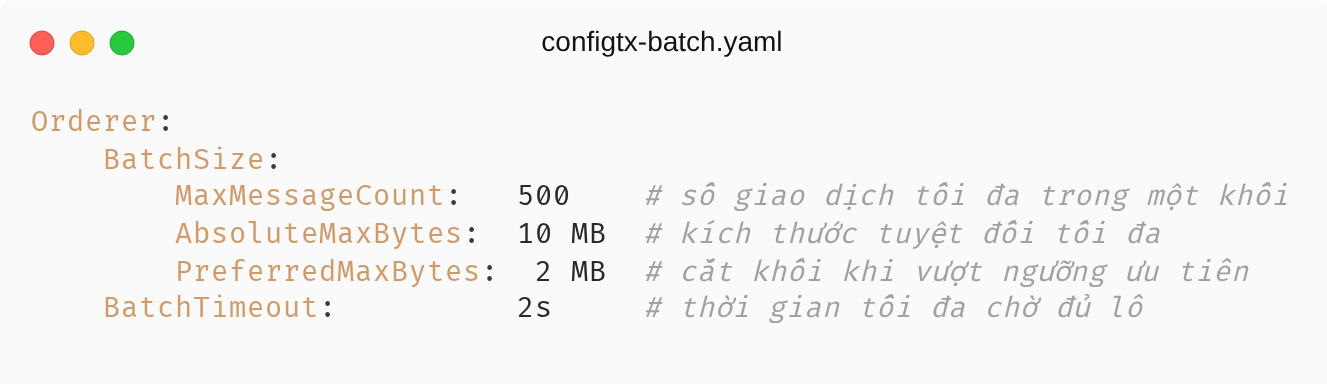
\includegraphics[width=0.75\textwidth, keepaspectratio]{Figures/code/configtx-batch.png}
    \caption{Cấu hình BatchSize và BatchTimeout trong configtx.yaml}
    \label{fig:configtx-batch}
\end{figure}

Một khối được đóng khi \textbf{thỏa một trong bốn điều kiện}: (1) số giao dịch đạt \pkg{MaxMessageCount}; (2) tổng kích thước vượt quá \pkg{AbsoluteMaxBytes}; (3) kích thước vượt quá ngưỡng \pkg{PreferredMaxBytes} (dù ngay cả khi chưa đủ \pkg{MaxMessageCount}); hoặc (4) \pkg{BatchTimeout} hết hạn dù lô chỉ có một giao dịch. Trong các điều kiện trên, \pkg{BatchTimeout} là yếu tố quyết định tính chất hành vi của mạng -- quyết định độ trễ chung quyết tối thiểu mà cử tri quan sát thấy. Cơ chế đóng khối được minh họa trong Hình~\ref{fig:batch-blockchain}.

\subsubsection{Đánh đổi giữa thông lượng và độ trễ}

Việc chọn \pkg{BatchTimeout} là một bài toán đánh đổi: tăng giá trị cho phép gom được nhiều giao dịch hơn vào một khối (tăng thông lượng), nhưng cử tri phải chờ lâu hơn để thấy phiếu được xác nhận. Bảng~\ref{tab:batch-timeout-tradeoff} tóm tắt ba kịch bản tham khảo.

\begin{table}[H]
\centering
\caption{Đánh đổi giữa BatchTimeout, thông lượng và độ trễ}
\label{tab:batch-timeout-tradeoff}
\begin{tabularx}{\textwidth}{|L{0.15}|L{0.25}|L{0.25}|L{0.35}|}
\hline
\textbf{Timeout} & \textbf{Thông lượng} & \textbf{Độ trễ} & \textbf{Phù hợp} \\
\hline
0.5 s & Thấp & Thấp (nhanh) & Hệ thống thời gian thực, ít người dùng \\
\hline
2 s & Trung bình & Trung bình & Cân bằng -- khuyến nghị cho bầu cử \\
\hline
5 s & Cao & Cao (chậm) & Nạp dữ liệu lớn, ít quan tâm độ trễ \\
\hline
\end{tabularx}
\end{table}

Với hệ thống bầu cử, \pkg{BatchTimeout = 2s} là điểm cân bằng phù hợp: 100 cử tri bỏ phiếu đồng thời có thể được gom vào cùng một khối, độ trễ chung quyết mà mỗi cử tri quan sát thấy nằm trong khoảng 2--3 giây -- đủ ngắn để giao diện ứng dụng cập nhật trạng thái phiếu mà không cần duy trì trạng thái chờ lâu, đồng thời đủ thông lượng để xử lý các đợt bỏ phiếu lớn.

\subsubsection{Phân biệt rõ giữa invoke và query}

Một tối ưu quan trọng ở tầng backend là \textbf{phân biệt nghiêm ngặt} giữa hai loại lời gọi chaincode: \textit{invoke} tạo ra giao dịch ghi và phải qua orderer để đóng khối; \textit{query} chỉ đọc dữ liệu trực tiếp từ World State của peer, không tạo giao dịch và không tốn quota khối. Bảng~\ref{tab:invoke-vs-query} liệt kê cách phân loại các hàm chaincode chính của hệ thống.

\begin{table}[H]
\centering
\caption{Phân loại các hàm chaincode theo invoke và query}
\label{tab:invoke-vs-query}
\begin{tabularx}{\textwidth}{|L{0.45}|L{0.15}|L{0.2}|L{0.2}|}
\hline
\textbf{Hàm chaincode} & \textbf{Loại} & \textbf{Tạo tx?} & \textbf{Độ trễ} \\
\hline
\pkg{SubmitVote}, \pkg{CommitMerkleRoot}, \pkg{RevealVoteCompact} & invoke & Có & 2--3 s \\
\hline
\pkg{GetVote}, \pkg{GetMerkleRoot}, \pkg{GetTally}, \pkg{GetAuditCounts}, \pkg{VerifyVoteReceipt} & query & Không & dưới 100 ms \\
\hline
\end{tabularx}
\end{table}

Việc sử dụng \pkg{query} cho mọi thao tác đọc -- tra cứu phiếu, kiểm tra gốc Merkle, tổng hợp kết quả -- giúp tải đọc của hệ thống không bao giờ chạm đến tầng đồng thuận, do đó không xung đột tài nguyên với tải ghi đang đợi đóng khối.
